\documentclass[a4paper,12pt,twoside]{report}
\usepackage{listings}
\usepackage{a4wide}
\usepackage{hyperref}
\usepackage[table]{xcolor}
\usepackage{booktabs}
\usepackage{pgfplots}
\usepackage{multirow}
\usepackage{pgfplotstable}
\usepackage{filecontents}
\usepackage{amsmath}
\usepackage{tikz}
\usepackage{gensymb}
\usepackage{forest}
\usepackage{pbox}
\usepackage[final]{pdfpages}
\usepackage[utf8]{inputenc}

\usepackage{graphicx}
\graphicspath{ {images/}}
\usepackage{float}

\usepackage{fancyhdr}
\pagestyle{fancy} %TODO: Headers need work

\parindent 0pt
\parskip 6pt
\pagenumbering{Roman}


\pgfplotstableread[col sep=comma]{./data/eval-desc-icon.csv}\icondesctable
\makeatletter
\pgfplotsset{
    /pgfplots/flexible xticklabels from table/.code n args={3}{%
        \pgfplotstableread[#3]{#1}\coordinate@table
        \pgfplotstablegetcolumn{#2}\of{\coordinate@table}\to\pgfplots@xticklabels
        \let\pgfplots@xticklabel=\pgfplots@user@ticklabel@list@x
    }
}
\makeatother


\begin{document}

%%%%%%%%%%%%%%%%%%%%%%%%%%%%%%%%%%%%%%%%%%%%%
% Macros
\newcommand{\todo}[1]{{\color{red} TODO: {#1}}}
\newcommand{\note}[1]{{\color{blue} NOTE: {#1}}}
\newcommand{\imageplaceholder}[3][Placeholder Image]{
  \begin{figure}[H]
    \centering
    \includegraphics[width=#2,height=#3]{pixel.png}
    \caption{#1}
  \end{figure}
}
\newcommand{\rot}[1]{\rotatebox{90}{#1}}

\begin{titlepage}
%%%%%%%%%%%%%%%%%%%%%%%%%%%%%%%%%%%%%%%%%%%%%%
% Title Page

\newcommand{\HRule}{\rule{\linewidth}{0.5mm}} % Defines a new command for the horizontal lines, change thickness here

%----------------------------------------------------------------------------------------
%	AUTHOR
%----------------------------------------------------------------------------------------

\begin{flushright} \large
Roman \textsc{Kolacz}\\
rk476@cam.ac.uk
\end{flushright}
\hspace{2cm}
\center % Center everything on the page
 
%----------------------------------------------------------------------------------------
%	HEADING SECTIONS
%----------------------------------------------------------------------------------------

\textsc{\LARGE University of Cambridge}\\[1.5cm] % Name of your university/college
\textsc{\Large Computer Science Tripos}\\[0.5cm] % Major heading such as course name
\textsc{\large Part II Project}\\[0.5cm] % Minor heading such as course title

%----------------------------------------------------------------------------------------
%	TITLE SECTION
%----------------------------------------------------------------------------------------

\HRule \\[0.4cm]
{ \huge \bfseries Time-Lapse Based Weather Classification}\\[0.1cm] % Title of your document
\HRule \\[1.5cm]
 
%----------------------------------------------------------------------------------------
%	DATE SECTION
%----------------------------------------------------------------------------------------

{\large 2014-2015}\\[3cm] % Date, change the \today to a set date if you want to be precise

%----------------------------------------------------------------------------------------
%	LOGO SECTION
%----------------------------------------------------------------------------------------

\includegraphics[height=7cm]{stp.jpg}\\
 
%----------------------------------------------------------------------------------------

\vfill % Fill the rest of the page with whitespace

\end{titlepage}

The landscape on the cover is of Saint Petersburg, Russia. It was taken with a drone, and shows an unexpected spell of sunshine illuminating The Church of the Saviour on Spilled Blood during a brewing storm.

Saint Petersburg is the birth place of Wladimir K\"{o}ppen (1846-1940), who developed the \textit{K\"{o}ppen Climate Classification System}. It is the most widely used weather classification system to this day.
\vfill

\chapter*{Proforma}
\setcounter{page}{1}
%%%%%%%%%%%%%%%%%%%%%%%%%%%%%%%%%%%%%%%%%%%%%%
% Proforma, table of contents, list of figures

\begin{tabular}{ll}
  \bf Name: & Roman Kolacz \\
  \bf College: & Downing College \\
  \bf Project Title: & Time-Lapse Based Weather Classification \\
  \bf Examination: & Computer Science Tripos - Part II \\
  \bf Word Count: & $\approx 8000$ \\
  \bf Project Originator: & Alan Blackwell \\
  \bf Project Supervisor: & Advait Sarkar \\
\end{tabular}

\section*{Initial Project Aims}
The initial aim of the project was to associate time-lapse video with external data sources by using a time-lapse video of an outside location to tell the weather. This would then be evaluated against real weather information and demonstrated graphically.

\section*{Work Completed}
Over a months worth of data (10,527 data points at 5 minute intervals), has been gathered. A classifier has been built which uses extracted image metrics and actual weather data to train a machine learning classifier which can then infer the weather.
The accuracy of several machine learning algorithms has been tested and the best for each data set has been used to maximise overall accuracy. 
The plan was changed from using manually hard-coded rules for weather classification to using machine learning to do so instead.

\section*{Special Difficulties}
A total of three Raspberry Pi's were used over the course of the data gathering stage, due to malfunctions and unfortunate mishaps. These significantly delayed the data gathering stages of the project, resulting in less data being gathered than planned.

\section*{Declaration of Originality}
I, Roman Kolacz of Downing College, being a candidate for Part II of the Computer Science Tripos, hereby declare that this dissertation and the work described in it are my own work, unaided except as may be specified below, and that the dissertation does not contain material that has already been used to any substantial extent for a comparable purpose.

\bigskip
\leftline{\bf Signed:}

\bigskip
\leftline\bf{\bf Date:}

\newpage

\section*{Acknowledgements}
Alan Blackwell, for help with the initial project idea and with directing the idea towards one which was suitable to use as a Part II project.

Advait Sarkar, for all his help and guidance as a supervisor and  without whom this dissertation would not have been possible.

\tableofcontents

\listoffigures

\listoftables

%%%%%%%%%%%%%%%%%%%%%%%%%%%%%%%%%%%%%%%%%%%%%%
% Dissertation content
\chapter{Introduction}\pagenumbering{arabic}
This dissertation aims to describe the process of building, testing and evaluating a weather classifier from time-lapse video, including the process of gathering the data necessary to train such a classifier. 

The dissertation will be split into three main chapters: Preparation, Implementation and Evaluation.

The preparation chapter will largely focus on data gathering and research undertaken to allow the project to proceed smoothly. This involved using hardware to take images and gather local weather data at regular intervals, while the research included reading around approaches to similar problems in the past, as well as learning about the algorithms and libraries which would be employed in the project.

The implementation chapter will go into detail on how a classifier was built to use the data gathered to classify the weather. It will describe the process of extracting features from the images gathered, and how the data was stored to then be used by the machine learning library. It will then detail how the data was used to train, run and test the classifier. 

The evaluation chapter will then focus on the results obtained from the classifier built in the previous section. This will include how it was tested, the overall accuracy of the classifier, and comparisons between different machine learning algorithms for different measures of weather conditions.

\section{Motivation}
Time lapse videos are a relatively unexplored aspect of data visualisation, and have a rather unique property amongst video of being able to hold information about incredibly large periods of time in a relatively small amount of time and space, provided they are of an event which occurs slowly and gradually, or is otherwise relatively uneventful.

An example of such an event is weather changes, including day-night transitions. These can very reliably be captured using time-lapse video as there are only minor changes between frames and the events are relatively long, so a constant video stream would be unnecessary and would result in either a long uninteresting video, or a very large proportion of wasted frames should the video be sped up to a watchable speed.

Weather classification was one particular example of associating time-lapse videos with external data sources, though a very similar approach could be used for other data, such as time-lapse videos mounted to tourist locations to observe places of interest and `hotspots' over different periods of time.

Weather has a vast and often understated impact on modern life. Weather variability cost the U.S economy an estimated \$485billion in 2008\cite{econweather}, though it also undeniably affects even the smallest of decisions in peoples day to day lives (such as whether sunglasses or an umbrella should be taken for the journey to work). As such, weather classification and prediction has become an all but essential area of research, with the capacity to greatly impact the world.

\section{Challenges}
Numerous challenges had to be considered before work on the project began.

One such challenge was deciding which features from within an image should be extracted to maximise classifier accuracy. This involved finding the features with large differences between classes to ease classification and with minimum inter-class variance to decrease false classification rates.

Another challenge to be circumvented was how similar looking weather conditions would be differentiated, given the features extracted. An example of such conditions would be heavy snow and direct sunlight (in that the image would be largely filled with white), or fog and rain.

Thirdly, as an experiment, temperature was added despite there being few visual cues in an image which would accurately depict the temperature. This was especially the case in England where sub 10\celsius{} temperatures in direct sunlight (a visual cue generally associated with warmth) and rain or dark clouds (generally associated with coldness) on a warm day were not uncommon occurrences.

\section{Related Work}
A number of previously published papers were useful for learning about various aspects of the project.

An approach which forms the basis of the weather-labelling per frame is described in
the paper ``Classification of Weather Situations on Single Colour Images''\cite{4621205}. It 
describes classifying weather using image metrics to be used to assist driving-assistance
systems which are heavily dependent on clear conditions. It achieves very accurate results
using only two labels (clear and rain), and reasonable accuracy when adding a third,
``light rain'' label. This project will build on this by adding further labels to the weather
classifying, as well as incorporating a cloud-cover measure.

The paper also mentions inaccuracies relating to weather situations containing heavy fog
or rain, as visibility is greatly reduced. These would have to be taken into consideration.

Another paper referenced is ``Support Vector Machines for Histogram-Based Image Classif-
ication''\cite{788646}, which describes that classification using support vector machines (and thus classification generally) is possible using only high dimensional histograms, whilst the paper
``Image Classification using Random Forests and Ferns''\cite{4409066} describes classifying images using Random Forests. This project will aim to incorporate aspects from both papers, in that it will be using Random Forests (alongside other classifiers) with mainly high dimensional histograms as feature set.

Although unrelated to weather classifying, ``Time-Lapse Photography Applied to Educa-
tional Videos''\cite{6202303} explores applying time-lapse videos to educational videos to aid with
analysing long term trends and discarding short term `noise'. This is comparable to what
this project is aiming to achieve through the use of time-lapse video.


\section{Related Courses}
The project builds upon the following courses from the Computer Science Tripos,
\begin{enumerate}
	\item Artificial Intelligence 
	\item Information Theory and Coding
	\item Algorithms
	\item Software Engineering
	\item Computer Vision
	\item Programming in Java and Further Java
\end{enumerate}

Additional reading and research on machine learning algorithms, feature extraction and data management were also carried out to make the project possible.
\chapter{Preparation}

This chapter will go into detail on the hardware used to gather data, the theoretical background behind the Random Forest and Multilayer Perceptron machine learning algorithms, and an explanation behind the choices made with regards to which tools to use throughout the project.

\section{Requirements Analysis}

\renewcommand\H{\multicolumn{1}{>{\columncolor{red!30}[9pt]}c}{H}}
\newcommand\M{\multicolumn{1}{>{\columncolor{yellow!30}[9pt]}c}{M}}
\renewcommand\L{\multicolumn{1}{>{\columncolor{green!30}[9pt]}c}{L}}

\begin{table}[H]
    \centering
    \setlength{\tabcolsep}{1em}
    \begin{tabular}{l ccc}
		\toprule
        \textbf{Component} & \textbf{Risk} & \textbf{Priority} & \textbf{Difficulty} \\[0.1cm]
		\midrule
        Data Gathering \\
		\cmidrule(r){1-1}
        Set up image gathering hardware & \H & \H & \M \\
        Understand Forecast.io API & \L & \M & \L \\
        Set up file-backup & \L & \L & \L \\
        Implement data gathering & \M & \H & \M \\
        \cmidrule(r){1-1}
        Classification \\
		\cmidrule(r){1-1}
        Implement feature extraction & \M & \H & \H \\
        Understand WEKA API & \L & \M & \M \\
        Implement classification & \M & \H & \H \\
        Try different algorithms & \L & \L & \M \\
        \cmidrule(r){1-1}
        Evaluation \\
		\cmidrule(r){1-1}
        Describe gathered data & \L & \H & \L \\
        Implement cross validation & \M & \M & \M \\
        \bottomrule
    \end{tabular}
    \caption{Requirements breakdown}
    \label{require}
    Values are High (H), Medium (M) and Low (L).
\end{table}
The project was split into key components, which were then assigned values for how much risk, priority and difficulty they carried with them (as shown in figure \ref{require}. High risk components had a large chance of failing early, or had failures which were difficult to recover from should they occur. High priority components were integral to the success of the project, and often had other components depend on them. Difficult components were likely to require a large amount of time and resource investments to get working to satisfactory standards. Development of components with high values in any of the three attributes was prioritised.

The Spiral software development model was used, as it allowed for frequent testing and sudden changes to be made throughout the course of the project. This was particularly useful as the exact requirements and specifications of the project were often only realised once development had begun.

\section{Data Gathering}
Due to the requirement of a large set of time constrained data, data gathering was a high priority to get under way and working as soon as possible. Every 5 minutes which passed was an image not taken and thus a data point lost (as although past weather information was available, an image from the past was not practical to obtain or emulate).

The data gathering involved using a small hardware setup to gather images and real weather information and then storing it in an easy to use, easy to read format.

\subsection{Hardware}
The Raspberry Pi\cite{RPi} is a small, credit-card sized computer created with the intention of aiding the teaching of Computer Science to young children. The device is small, cheap and can run Linux, which makes it excellent for small hardware applications such as for what was required by this project.

A `Model B' Raspberry Pi was used for the project. It has a 700MHz ARM CPU, a dedicated Broadcom VideoCore GPU and 512 MB of shared RAM\cite{pispecs}.

A Camera Module\cite{RPiCam} is also available for the Raspberry Pi, which plugs into a dedicated port on the Pi using a flat cable, and can shoot 1080p video or take up to 5 megapixel photographs. Although the Camera Module software bundled includes a time-lapse command to automatically generate time-lapse video, a Java program was instead made to take the images as further actions such as weather querying and uploading also needed to be carried out on each interval.

A Raspberry Pi with the Camera Module was used to take pictures at a 5 minute interval out of a window overlooking the Downing College court.

\begin{figure}[H]
 \centering
 \begin{tikzpicture}
   \node[anchor=south west,inner sep=0] (image) at (0,0) {\includegraphics[scale=0.6]{prep-setup.png}};
   \begin{scope}[x={(image.south east)},y={(image.north west)}]
     \draw[dashed,latex-,line width=2pt] (0.65,0.69) -- (1.05, 0.9)node[anchor=west,text width=4cm,black]{Camera module};
     \draw[dashed,latex-,line width=2pt] (0.5,0.5) -i (1.05, 0.7)node[anchor=west,text width=4cm,black]{Tape to hold setup in place};
     \draw[dashed,latex-,line width=2pt] (0.77,0.4) -i (1.05, 0.5)node[anchor=west,text width=4cm,black]{Raspberry Pi in clear enclosure};
 \end{scope}
 \end{tikzpicture}
 \caption{The Raspberry Pi and Camera Module Setup} 
\end{figure}

At each interval, data was added to a file which contained the necessary image metrics to train the classifier, as well as actual weather data and basic file information such as the name, date and time.
This file, along with each image, was then uploaded to an online file sharing platform so it could be accessed from other devices which required the gathered data. This is explored in more detail in section \ref{sec:datastoring}.

\section{Time Lapse}
Time-lapse video worked especially well for this project, as using a camera placed in a single location for the duration of the data gathering ensured that variables which would adversely impact the features extracted were kept constant. Using images taken from different places would have a different visibility of the sky, and would've contained different lighting features and shadows as well as different objects which would likely be differently coloured. These would be unideal for the purpose of training a classifier.
Given that the images were taken at regular intervals from a single location, time-lapse video was a logical next step.

Time-lapse involves taking photographs at regular (variable length, generally no more than a few minutes though can be as often as a few seconds) intervals which when played at a standard frame rate (30-60 FPS) look like time is sped up significantly. In this project, the interval was set at 5 minutes, which gives about two and a half hours of real-world time for every second of video when played at a standard 30 FPS.

\section{Machine Learning}
Research was devoted towards learning how different machine learning algorithms can be used and which would excel in different parts of the weather classification system.

\subsection{Random Forest}
A decision tree in machine learning is a tree-like structure which can be utilised to reach a conclusion based on a given set of parameters. At each branch, a path is chosen based on a condition, and the tree is traversed in this way until a leaf is reached with an outcome. 

Decision trees are simple to generate and use. Unfortunately, they have a high variance as even small changes in inputs can cause the traversal of different branch paths to drastically different results. They also have a tendency to over fit data (so outliers are significantly accounted for and general patterns are not formed) when trained too much, and are thus not usable as a reliable machine learning algorithm without modifications. They are however, used as building blocks for many other machine learning algorithms, one of which being the Random Forest.

\begin{figure}[H]
 \centering
 \tikzstyle{block}=[rectangle, draw, text width = 5em, text centered, rounded corners, minimum height = 3em]
\tikzstyle{block question}=[block, fill=red!20]
\tikzstyle{block answer}=[block, fill=blue!20]
\tikzstyle{blocklabel}=[midway]

\begin{forest}
	[Is average brightness higher than 75\%?, block question
		[Is contrast high?, block question, edge label={node[blocklabel, left]{yes}}
        	    [Sun, block answer, edge label={node[blocklabel, left]{yes}}]
        	    [Snow, block answer, edge label={node[blocklabel, right]{no}}]		
		]
		[Is average hue blue?, block question, edge label={node[blocklabel, right]{no}}
		    [Rain, block answer, edge label={node[blocklabel, left]{yes}}]
		    [Cloud, block answer, edge label={node[blocklabel, right]{no}}]
	    ]
    ]
\end{forest}

 \caption{A basic example decision tree for classifying the weather from an image}
\end{figure}

Decision tree training involves creating branches based on the best splits of data at each stage, such that the uncertainty at each node is minimised. This is obtained by maximising Information Gain, a variable which calculates the difference in entropy (a value used to measure the impurity of a set of random variables) of a set of data given a selected attribute to split the data against.

In a set of training data defined by 
$$T = \{(\mathbf{x}_1, y_1), \cdots, (\mathbf{x}_n, y_n) \}$$
where $\mathbf{x} = \{x_1, \cdots, x_n\}$ is the set of attributes and $y$ is the desired result of a value with the given attributes.

The entropy of a data set is defined by
$$H(T) = -\sum_{i=1}^{|T|} P(y_i)\log_2 P(y_i)$$
Where $P(t)$ is the probability mass function of $T$.

Information Gain over the $a$\textsuperscript{th} attribute is then defined by 
$$IG(T, a) = H(T) - \sum_{v \in vals(a)} \frac{|T_{a,v}|}{|T|}H(T_{a,v})$$
where $T_{a,v}$ is the subset of $T$ whose members contain value $v$ in the $a$\textsuperscript{th} attribute, defined by
$$T_{a,v} = \{\mathbf{x} \in T | x_a = v\}$$

The trees are then created top-down by selecting the attribute with maximum information gain at each branch.

A random forest is a machine learning algorithm which builds upon decision trees and corrects for their variance and tendency to over fit. It works by using multiple decision trees each trained on randomly selected data points from the training set which individually classify the data. Although individual trees may overfit or be sensitive to outliers, the trees overall tend to have little to no correlation and thus tend not to overfit the data.

Either the mode (for classification) or the mean (for regression) of the results of the individual trees is used as the final outcome.

\begin{figure}[H]
  \centering
  \tikzstyle{node}=[circle, draw, minimum size=13pt]
\tikzstyle{untaken node}=[node, fill=blue!30]
\tikzstyle{taken node}=[node, fill=red!50,]
\begin{forest}
[Input
	[,taken node, edge={->, draw, line width=1pt, black}
		[,taken node, edge={->, draw, line width=1pt, red}
			[,untaken node
			    [,untaken node]
			    [,untaken node]		
			]
			[,taken node, edge={->, draw, line width=1pt, red}
			    [,taken node, edge={->, draw, line width=1pt, red}, name=x1]
			    [,untaken node]			
			]
		]
		[,untaken node
			[,untaken node
			    [,untaken node]
			    [,untaken node]			
			]
			[,untaken node
			    [,untaken node]
			    [,untaken node]		
			]
		]
	]
	[,taken node, edge={->, draw, line width=1pt, black}
		[,untaken node
			[,untaken node
			    [,untaken node]
			    [,untaken node]		
			]
			[,untaken node
			    [,untaken node]
			    [,untaken node]		
			]
		]
		[,taken node, edge={->, draw, line width=1pt, red}
			[,taken node, edge={->, draw, line width=1pt, red}
			    [,untaken node]
			    [,taken node, edge={->, draw, line width=1pt, red}, name=x2]		
			]
			[,untaken node
			    [,untaken node]
			    [,untaken node]		
			]
		]
	]
	[,taken node, edge={->, draw, line width=1pt, black}
		[,untaken node, edge={->, draw, line width=1pt, red}
			[,untaken node, edge={->, draw, line width=1pt, red}
			    [,untaken node, edge={->, draw, line width=1pt, red}, name=x3
				[$\sum$, draw, edge={->, draw, line width=1pt}, name=end, before drawing tree={x=0.5,y=-7cm}
					[Output, edge={->, draw, line width=1pt}, before drawing tree={x=0.5,y=-8cm}]
				]
			    ]
			    [,untaken node]		
			]
			[,untaken node
			    [,untaken node]
			    [,untaken node]		
			]
		]
		[,untaken node
			[,untaken node
			    [,untaken node]
			    [,untaken node]		
			]
			[,untaken node
			    [,untaken node]
			    [,untaken node]		
			]
		]
	]
    ]
]
\draw[->, line width=1pt](x1)--(end);
\draw[->, line width=1pt](x2)--(end);
\end{forest}

  \caption{Random Forest with three trees}
\end{figure}

Random forests run relatively quickly and thus were used from an early stage in the project to see if classification was working and to give a rough estimate of the overall accuracy of classification (primarily to see if it was better than randomly guessing the weather).

\subsection{Multilayer Perceptron}
A single perceptron simply returns a value between 0 and 1 based on a given input and a given activation function. Two of the more commonly used activation functions are the threshold function, defined by

$$f(x)=\left\{ 
  \begin{array}{ll}
    1 & \quad \text{if } x \geq 0 \\
    0 & \quad \text{otherwise}\\
  \end{array}\right.$$
And the logistic function, defined by 
$$f(x) = \frac{1}{1 + e^{-x}}$$

Where $x$ is the output of the perceptron function defined by
$$Y = \mathbf{x} \cdot \mathbf{w} + b$$
In which $Y$ is the output of the perceptron, $\mathbf{x}$ is an input vector, $\mathbf{w}$ is the weight vector and $b$ is a constant term independent of the inputs.
This can be simplified to simply 
$$Y = \mathbf{x} \cdot \mathbf{w}$$
By treating the constant term, $b$ as another element in the input and weight vectors.

It aims to divide the data into two sets- the number returned determines which side of the division the given value should lie, and does so by recursively comparing its output with the desired output and adjusting the weights and bias' accordingly.

A multilayer perceptron uses at least three layers of perceptrons: input, output and at least one layer in between, known as the hidden layer. Each individual perceptron in each layer connects with a certain weight to every perceptron in the following layer. The final layer (the output layer) contains only one perceptron so that only one output value is obtained.

\begin{figure}[H]
  \centering
  \input{./snippets/mlp3.tex}
  \caption{Three layer multilayer perceptron}
\end{figure}

The output of each perceptron in a layer other than the input layer in this case is 
$$Y_{n,j} = f(\sum_{i=0} (Y_{n-1,i} \cdot w_{n,i,j}))$$
Where $Y_{n,j}$ is the output of a given perceptron in layer $n$ and position $j$, $w_{n,i,j}$ is the weight of the output from layer $n-1$ at $i$ to layer $n$ at $j$ and function $f$ is the activation function as detailed above.

A multilayer perceptron is trained in a similar way to a single perceptron. The weights of the connections are changed to adjust the acquired value to the expected value in the training set, and this is done backwards through the layers and then recursively over the entire network.

\begin{figure}[H]
  \centering
  \def\layersepp{2.5cm}
\def\layerseppp{5cm}
\def\layersepppp{7.5cm}
\begin{tikzpicture}[shorten >=1pt,->,draw=black, node distance=\layersepp]
    \tikzstyle{every pin edge}=[<-,shorten <=1pt]
    \tikzstyle{neuron}=[circle, draw,minimum size=13pt]
    \tikzstyle{input neuron}=[neuron, fill=red!50];
    \tikzstyle{output neuron}=[neuron, fill=green!30];
    \tikzstyle{hidden neuron}=[neuron, fill=blue!30];
    \tikzstyle{annot} = [text width=4em, text centered]

    % Draw the input layer nodes
    \foreach \name / \y in {2,...,5}
    % This is the same as writing \foreach \name / \y in {1/1,2/2,3/3,4/4}
        \node[input neuron, pin=left:] (I-\name) at (0,-\y) {};

    % Draw the hidden1 layer nodes
    \foreach \name / \y in {1,...,7}
        \path[yshift=0.5cm]
            node[hidden neuron] (H1-\name) at (\layersepp,-\y cm) {};

    % Draw the hidden2 layer nodes
    \foreach \name / \y in {2,...,6}
        \path[yshift=0.5cm]
            node[hidden neuron] (H2-\name) at (\layerseppp,-\y cm) {};

    % Draw the hidden3 layer nodes
    \foreach \name / \y in {1,...,7}
        \path[yshift=0.5cm]
            node[hidden neuron] (H3-\name) at (\layersepppp,-\y cm) {};

    % Draw the output layer node
    \node[draw, output neuron,pin={[pin edge={->}]right:Output}, right of=H3-4] (O) {};

    % Connect every node in the input layer with every node in the
    % hidden layer.
    \foreach \source in {2,...,5}
        \foreach \dest in {1,...,7}
            \path (I-\source) edge (H1-\dest);

    \foreach \source in {1,...,7}
        \foreach \dest in {2,...,6}
            \path (H1-\source) edge (H2-\dest);

    \foreach \source in {2,...,6}
        \foreach \dest in {1,...,7}
            \path (H2-\source) edge (H3-\dest);

    % Connect every node in the hidden layer with the output layer
    \foreach \source in {1,...,7}
        \path (H3-\source) edge (O);

    % Annotate the layers
    \node[annot,above of=H2-2, node distance=2cm] (t1) {Hidden layers};
    \node[annot,left of=t1, node distance=5cm] {Input layer};
    \node[annot,right of=t1, node distance=5cm]{Output layer};
\end{tikzpicture}

  \caption{Five layer multilayer perceptron}
  \label{fivemlp}
\end{figure}

Multilayer perceptrons tend to have multiple layers, and each layer can have any amount of perceptrons in it. Figure \ref{fivemlp} shows a 5 layer MLP with 7, 5 and 7 nodes in its respective hidden layers.

\section{Choice of Tools}
\subsection{Programming Language}
Java was used for the entirety of the project. It was chosen to ease development across different operating systems and to be able to use the WEKA library.

Performance wasn't an issue as the classifying was done in a single run whenever results were required, rather than dynamically with the data gathering (few machine learning algorithms support dynamic training in this way even if it were to be undertaken). Performance of individual classifiers is discussed in greater detail in section \ref{sec:performance}. 

\subsection{Libraries}
\subsubsection{WEKA}
The WEKA\cite{Hall:2009:WDM:1656274.1656278} library was used for machine learning. It provides the functionality to train its classifiers on CSV files with whatever options need to be set. 

The API\cite{wekaapi} contains features which can be split into three categories:
\begin{enumerate}
  \item Preprocessing
  \item Training
  \item Classifying
\end{enumerate}

The preprocessing classes include classes for managing data contained within CSV and ARFF (Attribute-Relation File Format) files, or databases; and preparing them to be used with the classifiers. Amongst them are included options for setting input attributes and the desired result column, as well as options for managing attributes by converting between continuous and discrete types or simply removing them altogether.

The training classes include the multitude of classifiers and options WEKA comes with, including Random Forests, Multilayer Perceptrons, J48, along with many others which weren't used for this project.

Once a classifier has been trained, WEKA provides functionality for providing an output based on a set of attributes. The CSV files were then modified with separate code to create columns with the results so that each row could be individually used for comparisons.


\subsubsection{Forecast.io}
The Forecast.io\cite{forecast} API was used for gathering the ground truth weather data. It provides an accurate forecast based on longitude and latitude for all the data which was required, and more. Forecast.io allows 1,000 free queries daily, which is above the amount required for the 5-minutely querying of the project.

Forecast.io uses a wide range of data sources including the USA NOAA System\cite{noaa}, the UK Met Office\cite{metoffice} and various worldwide meteorological reports. The data gathered is statistically aggregated to provide the most accurate data available.

The Forecast.io API takes a longitude and latitude and returns a JSON file with detailed weather information subdivided into minutely, hourly and daily; each of which contain data for several units of time (60 minutes, 48 hours and 7 days, respectively) in either past or future directions. A wrapper\cite{fiowrap} library was used to deserialize the JSON format into classes with the relevant data.
For this project, the current weather data rather than forecasted or historical weather data was used, so the information was only gathered when the image was taken.

Unfortunately, visibility as a column had to be omitted because Forecast.io didn't provide real visibility data for the area.

\subsection{Backups}
Dropbox\cite{dropbox} and GitHub\cite{git} were both used to ensure the project was safe should my hard drive become inaccessible. 
This was done by creating the git repository within a dropbox folder. Versioning and branching wasn't used due to the linear nature of the project and the fact that the work was done by a single person on a single computer at a time.

\chapter{Implementation}
\begin{figure}[!htb]
  \centering
  \tikzstyle{block} =[rectangle, draw, fill=blue!20, text width = 5em, text centered, rounded corners, minimum height = 4em]
\tikzstyle{line} = [draw, ->]

\begin{tikzpicture}[node distance = 2cm, auto]

  \node[block] (image) {Image Gathering};
  \node[block, below of = image] (feature) {Feature Extraction};
  \node[block, left of = feature, node distance = 3cm] (weather) {Weather Data Gathering};
  \node[block, below of = weather, xshift = 1.5cm] (storing) {Data Storing};
  \node[block, below of = storing] (training) {Training Classifier};
  \node[block, below of = training] (cross) {Cross Validation};

  \path [line] (image) -- (feature);
  \path [line] (feature) |- (storing);
  \path [line] (weather) |- (storing);
  \path [line] (storing) -- (training);
  \path [line] (training) -- (cross);

\end{tikzpicture}

  \caption{Processing pipeline}
\end{figure}

\section{Gathering Image Data}

\subsection{Feature Extraction}
Once the images had been obtained with the hardware detailed above, the features had to be extracted in order to train the classifier. Initially OpenCV\cite{opencv} was going to be used, though soon into development there was a realisation that there was little need for it and the feature extraction phase was implemented manually in Java.

The features to be extracted had to be chosen such that there was as much variation as possible between classes, and as little variation as possible within classes, to maximise classification accuracy. In addition to this, the features had to be easy to extract and store within a useable and easily readable format. 

The features extracted included:
\begin{itemize}
  \item Average Hue
  \item Brightness Histogram
  \item Each of the red, green and blue (RGB) histograms
\end{itemize}

These were obtained by sampling each pixel in the images using the Java BufferedImage\cite{bufferedimage} class to return the RGB values of the pixels of an image in sequence as an array of bytes.
The brightness value of a set of RGB values was determined by the luminance function.
$$Y = 0.2126R + 0.7152G + 0.0722B$$
where $Y$ is the luminance and $R$, $G$ and $B$ are Red, Green and Blue respectively.

This formula reflects how much each light contributes to the perceived brightness by a human eye\cite{Sutter1992433}. Green contributes the most, whereas blue contributes the least. Figure \ref{sunflower} shows how this method produces a better result than using the average of the RGB values\cite{sunflower}.

\begin{figure}[H]
  \centering
  \begin{tabular}{ccc}
  \includegraphics[scale=1]{sunflower-original.png} &
  \includegraphics[scale=1]{sunflower-luminance.png} &
  \includegraphics[scale=1]{sunflower-average.png} \\
  Original & Luminance & Average \\
  \end{tabular}
  \caption{Comparison of greyscale obtained via average and luminance methods}
  \label{sunflower}
\end{figure}

The histograms are a size 256 array containing the number of pixels with the given RGBY value.

The average hue was obtained by simply averaging the values of each of the pixels in each image.


\subsubsection{Examples of Images and Extracted Features}
Figures \ref{fig:rain} to \ref{fig:snow} show four examples of images taken during the data gathering stage, each with a different weather class. Even from an initial glance, several observations can be made.
\begin{enumerate}
  \item The picture of rain has a bluer tint due to the clouds and the refraction of the sky in the rain drops
  \item The picture with sunlight is highly contrasted due to the bright sky and deep shadows
  \item The picture of the night is darker than the other images, and should thus have a significantly lower brightness. The specific weather conditions are, however, near impossible to tell.
  \item The picture with the snow is bright but significantly less saturated than the other images due to the greying effect of the snow on the image.
\end{enumerate}

\newpage % So that all four images are on two pages

\begin{figure}[H]
 \centering
 \includegraphics[scale=0.45]{imp-rain.png}
 \caption{An image taken during rain} 
 \label{fig:rain}
\end{figure}

\begin{figure}[H]
 \centering
 \includegraphics[scale=0.45]{imp-sun.png}
 \caption{An image taken during sunlight} 
\end{figure}

\begin{figure}[H]
 \centering
 \includegraphics[scale=0.45]{imp-night.png}
 \caption{An image taken during a cloudy night} 
\end{figure}

\begin{figure}[H]
 \centering
 \includegraphics[scale=0.45]{imp-snow.png}
 \caption{An image taken during snow} 
 \label{fig:snow}
\end{figure}

\begin{figure}[H]
  \centering
   \scalebox{0.92}{\begin{tabular}{cc}
  \begin{tikzpicture}
    \begin{semilogyaxis}[
      xlabel=Brightness,
      ylabel=Pixels,
      ylabel near ticks,
      xlabel near ticks,
      ymax=150000,
    ]
    \addplot[
      const plot,
      color=black,
      draw=black,
    ]
    table[x=x,y=rain-br,col sep=comma] {./data/prep-data.csv}; 
    \end{semilogyaxis}
    \node[align=center] at (3.5cm,5cm){Rain};
  \end{tikzpicture}&
  \begin{tikzpicture}
    \begin{semilogyaxis}[
      xlabel=Brightness,
      ylabel=Pixels,
      ylabel near ticks,
      xlabel near ticks,
      ymax=150000,
    ]
    \addplot[
      const plot,
      color=black,
      draw=black,
    ]
    table[x=x,y=sun-br,col sep=comma] {./data/prep-data.csv}; 
    \end{semilogyaxis}
    \node[align=center] at (3.5cm,5cm){Sun};
  \end{tikzpicture}\\
  \begin{tikzpicture}
    \begin{semilogyaxis}[
      xlabel=Brightness,
      ylabel=Pixels,
      ylabel near ticks,
      xlabel near ticks,
      ymax=150000,
    ]
    \addplot[
      const plot,
      color=black,
      draw=black,
    ]
    table[x=x,y=night-br,col sep=comma] {./data/prep-data.csv}; 
    \end{semilogyaxis}
    \node[align=center] at (3.5cm,5cm){Night};
  \end{tikzpicture}&
  \begin{tikzpicture}
    \begin{semilogyaxis}[
      xlabel=Brightness,
      ylabel=Pixels,
      ylabel near ticks,
      xlabel near ticks,
      ymax=150000,
    ]
    \addplot[
      const plot,
      color=black,
      draw=black,
    ]
    table[x=x,y=snow-br,col sep=comma] {./data/prep-data.csv}; 
    \end{semilogyaxis}
    \node[align=center] at (3.5cm,5cm){Snow};
  \end{tikzpicture}\\
  \end{tabular}
}

  \caption{Brightness histograms of all images}
  \label{fig:yhist}
\end{figure}
Figure \ref{fig:yhist} shows that the image of the cloudy night has far more pixels with lower brightness than the daylight images, making brightness a very effective feature to use with regard to determining night from day. Although more subtle, the image with the rain had a peak brightness significantly lower than the images of snow and sun, indicating that the brightness was overall lower than the other two images, though still significantly higher than with the night. Although the brightness could be used to split rain against sun and snow, there are likely to be more reliable features for doing so.

The histogram of brightness is likely to have high variance as images during midday are generally going to be brighter than images in the morning or evening (which would still be classified as day time). As such, general shapes of the graphs rather than exact values would need to be considered.

\begin{figure}[H]
  \centering
   \scalebox{0.92}{\begin{tabular}{cc}
  \begin{tikzpicture}
    \begin{semilogyaxis}[
      xlabel=Value,
      ylabel=Pixels,
      ylabel near ticks,
      xlabel near ticks,
    ]
    \addplot[
      const plot,
      color=red,
      unbounded coords = discard
    ]
    table[x=x,y=rain-r,col sep=comma] {./data/prep-data.csv}; 
    \addplot[
      const plot,
      color=blue,
      unbounded coords = discard
    ]
    table[x=x,y=rain-b,col sep=comma] {./data/prep-data.csv}; 
    \addplot[
      const plot,
      color=green,
      unbounded coords = discard
    ]
    table[x=x,y=rain-g,col sep=comma] {./data/prep-data.csv}; 
    \end{semilogyaxis}
    \node[align=center] at (3.5cm,5cm){Rain};
  \end{tikzpicture}&
  \begin{tikzpicture}
    \begin{semilogyaxis}[
      xlabel=Value,
      ylabel=Pixels,
      ylabel near ticks,
      xlabel near ticks,
      ymax=185000,
    ]
    \addplot[
      const plot,
      color=red,
      unbounded coords = discard
    ]
    table[x=x,y=sun-r,col sep=comma] {./data/prep-data.csv}; 
    \addplot[
      const plot,
      color=blue,
      unbounded coords = discard
    ]
    table[x=x,y=sun-b,col sep=comma] {./data/prep-data.csv}; 
    \addplot[
      const plot,
      color=green,
      unbounded coords = discard
    ]
    table[x=x,y=sun-g,col sep=comma] {./data/prep-data.csv}; 
    \end{semilogyaxis}
    \node[align=center] at (3.5cm,5cm){Sun};
  \end{tikzpicture}\\
  \begin{tikzpicture}
    \begin{semilogyaxis}[
      xlabel=Value,
      ylabel=Pixels,
      ylabel near ticks,
      xlabel near ticks,
      ymax=185000,
    ]
    \addplot[
      const plot,
      color=red,
      unbounded coords = discard
    ]
    table[x=x,y=night-r,col sep=comma] {./data/prep-data.csv}; 
    \addplot[
      const plot,
      color=blue,
      unbounded coords = discard
    ]
    table[x=x,y=night-b,col sep=comma] {./data/prep-data.csv}; 
    \addplot[
      const plot,
      color=green,
      unbounded coords = discard
    ]
    table[x=x,y=night-g,col sep=comma] {./data/prep-data.csv}; 
    \end{semilogyaxis}
    \node[align=center] at (3.5cm,5cm){Night};
  \end{tikzpicture}&
  \begin{tikzpicture}
    \begin{semilogyaxis}[
      xlabel=Value,
      ylabel=Pixels,
      ylabel near ticks,
      xlabel near ticks,
      ymax=185000,
    ]
    \addplot[
      const plot,
      color=red,
      unbounded coords = discard
    ]
    table[x=x,y=snow-r,col sep=comma] {./data/prep-data.csv}; 
    \addplot[
      const plot,
      color=blue,
      unbounded coords = discard
    ]
    table[x=x,y=snow-b,col sep=comma] {./data/prep-data.csv}; 
    \addplot[
      const plot,
      color=green,
      unbounded coords = discard
    ]
    table[x=x,y=snow-g,col sep=comma] {./data/prep-data.csv}; 
    \end{semilogyaxis}
    \node[align=center] at (3.5cm,5cm){Snow};
  \end{tikzpicture}\\
  \end{tabular}
}

  \caption{RGB histograms of all images}
  \label{fig:rgbhist}
\end{figure}
Figure \ref{fig:rgbhist} shows the histograms of the four example images (figures \ref{fig:rain} - \ref{fig:snow}). A logarithmic scale is used as the peaks are extreme and would flatten the rest of the graph with a linear scale.

As with the brightness histograms (figure \ref{fig:yhist}), the night images have large peaks for low values in all three colours, indicating an overall lack of brightness. 

The histograms are significantly different for each of the four images. Although the individual colour histogram shapes are generally very similar for the snow and sun images, the colours for the snow image are more strongly correlated, with peaks and troughs in almost identical places (as shown by the overlap in the lines). This indicates an overall balance of colours, and contrasts the sun image, which contains a high number of pixels with less red but has otherwise similar histograms for green and blue.

The blue histogram of the rain image distinguishes it the most from the other images due to the very large peak at around $210$ on the value axis. The red peak on the same image also occurs significantly later, and doesn't feature a drop off like the other images do. This trend is largely consistent between different images of the same weathers at different times of the day.

\begin{table}[H]
  \centering
  \begin{tabular}{ccc}
  \toprule
   Rain & & Sun \\
   \cellcolor[HTML]{7c808d}\texttt{(124, 128, 141)} & & \cellcolor[HTML]{8ea677}\texttt{(142, 166, 119)} \\
   \\
   Night & & Snow \\
   \cellcolor[HTML]{14171b}\color{white}\texttt{(20, 23, 27)} & & \cellcolor[HTML]{919590}\texttt{(145, 149, 144)} \\
  \bottomrule
  \end{tabular}
  \caption{The average hues of the images, shown as RGB values on a scale of 0 to 255}
\end{table}

The average hue of the image at night is incredibly dark due to the lack of sunlight. The sunlit image has a relatively bright green average hue, largely due to the grass which is in a large portion of the image. This is a feature which stays consistent throughout sunlit images which isn't present in other weather conditions.

The snow image also has a green hue to it, though is significantly less saturated than the sun image. This is caused by the whiteness of the snowfall and the snow or ice that settles or forms on the grass in the image.

The image of the rain has a blue hue to it, which contrasts with the green of the sun and snow images. The grass appears less vivid due to the obstruction of the sun by cloudy skies and  overall blue high can also be attributed to the refraction of the sky in the raindrops, as well as the overall darker blue hue of the sky itself. 

\section{Data Storing}
\label{sec:datastoring}
Comma-Separated Value (csv) files were used to store the data in a convenient way for both anyone reading the data and for the WEKA library. The data stored included the name of the image, the time and date it was taken, as well as the actual weather information occurring in the image and the features extracted to train a classifier. Blank columns were left for the predicted weather information which would be filled in by the classifier once it was trained.

The csv file was stored on the Dropbox file sharing platform. It was updated on every interval so that other devices could access a complete set of data immediately when required.

\begin{table}[H]
  \centering
  \scalebox{0.7}{

\begin{tabular}{cc}

\begin{tabular}{cccccccc}
  \toprule
  name & date & time & actual icon & $\cdots$ & actual temperature & predicted icon & $\cdots$\\
 2015-02-09T23:55.jpg & 2015-02-09 & 23:55:42 & cloudy & $\cdots$ & 3 & -- & $\cdots$\\
 2015-02-10T00:00.jpg & 2015-02-10 & 00:00:42 & cloudy & $\cdots$ & 3 & -- & $\cdots$  \\
 2015-02-10T00:05.jpg & 2015-02-10 & 00:05:42 & cloudy & $\cdots$ & 2 & -- & $\cdots$  \\
 2015-02-10T00:10.jpg & 2015-02-10 & 00:10:42 & cloudy & $\cdots$ & 2 & -- & $\cdots$  \\
 2015-02-10T00:15.jpg & 2015-02-10 & 00:15:42 & cloudy & $\cdots$ & 2 & -- & $\cdots$  \\
 2015-02-10T00:20.jpg & 2015-02-10 & 00:20:42 & cloudy & $\cdots$ & 2 & -- & $\cdots$  \\
 $\vdots$ & $\vdots$ & $\vdots$ & $\vdots$ & $\ddots$ & $\vdots$ & $\vdots$ & $\ddots$  \\
 \bottomrule
\end{tabular} & $\cdots$ \\
\\

\begin{tabular}{cccccccccccccc}
  \toprule
  predicted temperature & b[0] & $\cdots$ & b[255] & r[0] & $\cdots$ & r[255] & g[0] & $\cdots$ & g[255] & b[0] & $\cdots$ & b[255] & average hue \\
-- & 124552 & $\cdots$ & 0 & 329362 & $\cdots$ & 10 & 21685 & $\cdots$ & 367 & 210463 & $\cdots$ & 398 & \#0F090F \\
-- &  187945 & $\cdots$ & 2 & 302139 & $\cdots$ & 15 & 22310 & $\cdots$ & 347 & 248283 & $\cdots$ & 492 & \#0A0A0C \\
-- &  183065 & $\cdots$ & 7 & 312448 & $\cdots$ & 22 & 23409 & $\cdots$ & 629 & 223409 & $\cdots$ & 491 & \#09100D \\
-- &  169364 & $\cdots$ & 1 & 294123 & $\cdots$ & 14 & 24012 & $\cdots$ & 711 & 257234 & $\cdots$ & 572 & \#040E12 \\
-- & 10165 & $\cdots$ & 0 & 292341 & $\cdots$ & 12 & 21239 & $\cdots$ & 1 & 234829 & $\cdots$ & 481 & \#0F0511 \\
-- & 109382 & $\cdots$ & 1 & 290312 & $\cdots$ & 19 & 25010 & $\cdots$ & 25 & 242348 & $\cdots$ & 748 & \#0F590B \\
 $\vdots$ & $\vdots$ & $\ddots$ & $\vdots$ & $\vdots$ & $\ddots$ & $\vdots$ & $\vdots$ & $\ddots$ & $\vdots$ & $\vdots$ & $\ddots$ & $\vdots$ & $\vdots$ \\
 \bottomrule
\end{tabular} & 
\end{tabular}
}

  \caption{Example schema for csv file}
  (Split in half for ease of viewing)
\end{table}
 
\section{Sanity Checking}
Considering the high dependency of the project on the success and accuracy of the image gathering, it was vital to ensure that it was going smoothly. Although time-lapse footage exists which could otherwise have been used- the real weather information would have to be manually labelled on a frame by frame basis, which was impractical with so many data points.

Sanity checking ensures that everything is working, and if it isn't, that a user responsible is made aware as soon as possible to fix whatever problems may have arisen.

A sanity check which was employed in this project involved making sure that the Raspberry Pi was taking images and uploading them to dropbox continuously, as a large set of data was an integral part of the success of the project. The check employed confirmed that the real data was being gathered by querying the forecast.io API to ensure that weather information requests were occurring. This check did in fact come of use during the project, where a sudden disconnect in power supply from the Raspberry Pi due to cleaning meant that the existing error solutions built into the code did not have the chance to send an alert.

In addition to this, the main data gathering program was made to send an email alert should any exception be thrown throughout the image taking, data gathering, feature extraction and file saving/uploading stages. This provided a faster and more immediate notification when errors occurred than the sanity check detailed above.


\chapter{Evaluation}

\section{Cross Validation}
Cross validation is a technique used to evaluate machine learning algorithms by testing them on all of the dataset rather than using most of the data to train the algorithm and using only a small portion for testing. In this project, the data was divided into testing and training sets with a 1 to 4 ratio, respectively. This was done five times such that each of the testing sets were unique and formed the complete dataset, so each point of data was used to train four classifiers and was tested by one (which it didn't train).

It was important not to train and test the machine learning classifiers using the same data, as classifiers which remember instead of learn (such as any database store and lookup based algorithms) would perform disproportionately well.

\begin{figure}[H]
  \centering
  \begin{tabular}{ccc}
    \begin{tabular}{rp{0.3cm}p{0.3cm}p{0.3cm}p{0.3cm}p{0.3cm}}
    \toprule
    Iteration & \multicolumn{5}{c}{Data Split} \\
    1 & \cellcolor{red!30} & \cellcolor{blue!50} & \cellcolor{blue!50} & \cellcolor{blue!50} & \cellcolor{blue!50} \\
    2 & \cellcolor{blue!50} & \cellcolor{red!30} & \cellcolor{blue!50} & \cellcolor{blue!50} & \cellcolor{blue!50} \\
    3 & \cellcolor{blue!50} & \cellcolor{blue!50} & \cellcolor{red!30} & \cellcolor{blue!50} & \cellcolor{blue!50} \\
    4 & \cellcolor{blue!50} & \cellcolor{blue!50} & \cellcolor{blue!50} & \cellcolor{red!30} & \cellcolor{blue!50} \\
    5 & \cellcolor{blue!50} & \cellcolor{blue!50} & \cellcolor{blue!50} & \cellcolor{blue!50} & \cellcolor{red!30} \\
    \bottomrule
  \end{tabular} &  & \pbox{20cm}{\colorbox{blue!50}{\color{blue!50}AA} Train 
  \\ \colorbox{red!30}{\color{red!30}AA} Test}
\end{tabular}
  \caption{Cross Validation}
  \label{xval}
\end{figure}

The cross validation partitioning used is shown graphically in figure \ref{xval}. At each iteration, a different set is used for testing and the rest of the data is used to train the classifier. After all 5 iterations, each data point will have been used to train the classifier four times and test it once. More generally, the data can be divided into $k$ partitions such that the data set can be evaluated $k$ times by averaging results without the need for a larger dataset.

The partitions were allocated randomly to avoid trends which would've been present due to the ordering of the data.

\section{Description of Data}
The input data had to be analysed and described to give meaning to the evaluation. For the classification to be effective, the accuracy had to be higher than the mode of the data set; and for the regression based data, the root-mean-square error should have been within a standard deviation of the data.

\subsection{Weather Type}

\begin{figure}[htpb]
  \centering
  
  \begin{tikzpicture}
    \begin{axis}[
      ybar,
      xtick=data,
      ymin=0,
      ylabel=Percentage of Data,
      xlabel=Weather Type,
      xlabel near ticks,
      x tick label style={rotate=45, anchor=north east, inner sep=0mm},
      flexible xticklabels from table={./data/eval-desc-icon.csv}{icon}{col sep=comma},
    ]
    \addplot
    table[x expr=\coordindex,y=p]{\icondesctable};
    \end{axis}
  \end{tikzpicture}


  \caption{Distribution of weather types in the data set}
  \label{fig:descicon}
\end{figure}

There were initial concerns with how varied the weather type would be given the high likelihood of cloudy weather in the UK, especially during the period of data gathering. Fortunately, Forecast.io distinguishes between cloudy and partly cloudy, with the latter being further split into day and night classes. Due to this, the data is relatively spread out and a highly accurate classifier could not have been created by simply guessing cloudy all the time, as per the initial concerns.

Partly cloudy nights were still by far the most common type, with 32\% of the data points. The combined night values also account for 45\% of the data, which as expected, accounts for about half the data.

\subsection{Cloud Cover}
\begin{figure}[H]
  \centering
  \begin{tikzpicture}
    \begin{axis}[
      ymin=0,
	ylabel=Percentage of Data,
	xlabel=Cloud Cover (\%),
      xtick={0,20,...,100},
	ybar
    ]
    \addplot
    table[x=cover,y=p,col sep=comma]{./data/eval-desc-cloud.csv};
    \end{axis}
  \end{tikzpicture}
  \caption{Distribution of cloud cover percentages in the data set}
  \label{fig:desccloud}
\end{figure}

As figure \ref{fig:desccloud} shows, the cloud cover is distributed quite uniformly between 0\% (no cloud cover) and 100\% (complete cloud cover), with the mean and median being almost equal. By comparing this graph to the icon graph (figure \ref{fig:descicon}), it can be deduced that the `Partially Cloudy' cweather type classification occurs approximately between 20\% and 90\% cloud cover, and that cloudy occurs above 90\%. The standard deviation is 31\% cloud cover, so the classifier should aim to classify within that percentage.

\subsection{Precipitation}
\begin{figure}[H]
  \centering
  \begin{tikzpicture}
    \begin{axis}[
      ybar,
      ymin=0,
      xtick={0,1.06,...,4.57},
	ylabel=Percentage of Data,
	xlabel=Precipitation (mm),
    ]
    \addplot
    table[x=rain,y=p,col sep=comma]{./data/eval-desc-rain.csv};
    \end{axis}
  \end{tikzpicture}
  \caption{Precipitation data bar chart}
  
\end{figure}


Unlike the cloud cover, the precipitation is massively skewed toward the lower 10th percentile, which indicates that there was generally very little rain in the data gathering stage of the project. Over 97.4\% of the data was within the lowest percentile.

Although the standard deviation was a relatively low 0.23mm, a highly accurate approximation of the precipitation level can be made by simply guessing 0.23mm in all cases, which would be within a standard deviation of the actual value in over 90\% of the test cases. This is an unfortunate distribution, as the precipitation levels are not going to be a good indicator of classifier performance.

\subsection{Temperature}
\begin{figure}[H]
  \centering
  \begin{tikzpicture}
    \begin{axis}[
      ybar,
      ymin=0,
      xtick=data,
	xlabel=Temperature (\celsius),
	ylabel=Percentage of Data,
	xtick={0.24,3.09,...,13.07}
    ]
    \addplot
    table[x=temp,y=p,col sep=comma]{./data/eval-desc-temp.csv};
    \end{axis}
  \end{tikzpicture}
  \caption{Temperature data bar chart}
\end{figure}

The temperature is more distributed than the precipitation, though not as uniformly as the cloud cover. The data was gathered over the winter and early spring months, and so the temperature is generally very low with later dates having the higher temperatures. This would likely be a more uniform distribution if the data was to be taken over a longer period of time encompassing at least all four seasons. The average temperature was 6.08\celsius{} and there was a standard deviation of 2.9\celsius.

\subsection{Sunrise and Sunset}
The sunrise and sunset times changed predictably throughout the data gathering process to reflect on the increasing daylight hours as winter ended.
For the data as a whole, the standard deviation for the sunrise is 22 minutes whilst the standard deviation for the sunset is 19 minutes. These could likely be predicted with high accuracy if the time and dates were used as features to train the classifier. 

\section{Analysis of Classifiers}
The discrete data was analysed by simply comparing the percentage of correct classifications for each class.
The continuous data was analysed by calculating the root-mean-square error, given by
$$RMSE = \sqrt{\frac{\sum_{t=1}^n (x_t - y_t)^2}{n}}$$
where $x_t$ is the actual value and $y_t$ is the predicted value of the $t^{th}$ point of data in a set of $n$ data points.

\subsection{Random Forest}
Random forests were analysed with a varying number of trees ranging from 1 to 100, and also 200 and 1000. Results were obtained with each of the number of trees to analyse how performance changes for different classes with the increase in trees.

\subsubsection{Weather Type}
\begin{figure}[H]
  \centering
  \begin{tikzpicture}
    \begin{axis}[
      ymin=0,
	ylabel=Accuracy,
	xlabel=Number of Trees,
      xtick={1,2,3,4,5,6,7,8,9,10,11,12,13},
      xticklabels={1,10,20,30,40,50,60,70,80,90,100,200,1000},
      x tick label style={rotate=90, anchor=north east,yshift=2mm},
    ]
    \addplot
    table[x=x,y=p,col sep=comma]{./data/eval-rf-icon.csv};
    \end{axis}
  \end{tikzpicture}
  \caption{Weather type classification peformance per number of trees}
\end{figure}

The accuracy of the random forests increased significantly up to 50 trees, at which point it was 56.7\% accurate. From there, the accuracy fluctuated between a maximum of 57.3\% and a minimum of 55.2\%. The maximum performance of the random forest for this feature set was therefore realised between 40 and 50 trees.

57\% as an accuracy is good- well above randomly guessing and well above the mode value percentage, though still not accurate enough for any real world usage where potentially dangerous decisions can be influenced by weather.

\subsubsection{Sunrise and Sunset}
\begin{figure}[H]
  \centering
  \begin{tabular}{cc}
  Sunrise & Sunset \\
  \scalebox{0.92}{\begin{tikzpicture}
    \begin{axis}[
      ymin=0,
	ylabel=RMSE (seconds),
	xlabel=Number of Trees,
      xtick={1,2,3,4,5,6,7,8,9,10,11,12,13},
      xticklabels={1,10,20,30,40,50,60,70,80,90,100,200,1000},
      x tick label style={rotate=90, anchor=north east, yshift=2mm},
    ]
    \addplot
    table[x=x,y=rise,col sep=comma]{./data/eval-rf-sun.csv};
    \end{axis}
  \end{tikzpicture}}&
  \scalebox{0.92}{\begin{tikzpicture}
    \begin{axis}[
      ymin=0,
	ylabel=RMSE (seconds),
	xlabel=Number of Trees,
      xtick={1,2,3,4,5,6,7,8,9,10,11,12,13},
      xticklabels={1,10,20,30,40,50,60,70,80,90,100,200,1000},
      x tick label style={rotate=90, anchor=north east, yshift=2mm},
    ]
    \addplot
    table[x=x,y=set,col sep=comma]{./data/eval-rf-sun.csv};
    \end{axis}
  \end{tikzpicture}}\\
  \end{tabular}
  \caption{Sunrise and Sunset regression peformance per number of trees}
\end{figure}


There was no improvement in the accuracy of the prediction of sunrise as the number of trees increased, with the mean error continuously being about 30 minutes, which is over the standard deviation of 22 minutes, though still well within two standard deviations.

The sunset, as with the sunrise, also doesn't increase in accuracy as more trees are added to the forest. The average root-mean-square error of about 27 minutes is also outside of the standard deviation of 19 minutes, and for similar reasons to above, renders random forests a lacklustre way of predicting the sunset.

Given the algorithmic nature of sunset and sunrise times with respect to the day of the year, a significantly better set of results could be expected if the date was used as a feature.

To follow on this, sunrise and sunset times generally have little correlation with the features of individual images which were used to train the classifiers (it is almost impossible to tell when the sun will set from an image of a cloudy day). It is therefore unsurprising that the random forest classifier did not perform well for this class.

\subsubsection{Cloud Cover}
\begin{figure}[H]
  \centering
  \begin{tikzpicture}
    \begin{axis}[
      ymin=0,
      xtick={1,2,3,4,5,6,7,8,9,10,11,12,13},
      xticklabels={1,10,20,30,40,50,60,70,80,90,100,200,1000},
      x tick label style={rotate=90, anchor=north east, yshift=2mm},
	ylabel=RMSE (cloud cover \%),
	xlabel=Number of Trees,
    ]
    \addplot
    table[x=x,y=p,col sep=comma]{./data/eval-rf-cloud.csv};
    \end{axis}
  \end{tikzpicture}
  \caption{Cloud cover regression peformance per number of trees}
\end{figure}

From 10 trees onwards, the prediction of cloud cover did not increase in accuracy as the number of trees changed, staying at a root mean square error of about 32\% throughout the tests (and 40\% between 1 and 10 trees). This is almost exactly one standard deviation, and so Random Forests with at least 10 trees are accurate to an acceptable degree of error.

\subsubsection{Precipitation}
\input{./snippets/evaltreesrain.tex}
The precipitation prediction increased in accuracy as the number of trees increased, up to about a 0.17mm error, which is well within the 0.23mm standard deviation of the precipitation data. This performance was reached at about 40 trees, after which the performance changes were negligible as the number of trees increased.

Rather surprisingly, random forests are a rather good predictor of precipitation levels using the features that were extracted from the images.

\subsubsection{Temperature}
\input{./snippets/evaltreestemp.tex}
The temperature prediction did not increase in accuracy as the number of trees increased (with at least 10), though the root-mean-square error came to about 1.54\celsius, which is significantly under the standard deviation of 2.9\celsius. As such, rather surprisingly, random forests are not only quite good at inferring temperature from images, but more generally it is possible to infer temperature from an image to a relatively high degree of accuracy.
Of course, the temperature range of the data is rather limited (15\celsius) in terms of real-world temperature ranges, given the span of time of data gathering.

\subsubsection{Summary}
Overall, the Random Forest algorithm is generally the most successful, with very good results in predicting the weather type, temperature and precipitation, and with decent performance with the other classes.
All the classifications and regressions reached their maximum accuracy by 50 trees, with most of them taking only 10 before significant performance gains were no longer occurring.

\subsection{Multilayer Perceptron}

\subsubsection{Weather Type}
The multilayer perceptron had a 36.1\% accuracy rate with classifying the weather type. This is marginally better than assigning the mode result to every instance, and also better than the average case of randomly assigning types. However, this is by no means a reliable result for classifying the weather type as 36\% is a generally low success rate for classification (it's wrong more often than it's right). 

\subsubsection{Sunrise and Sunset}
The sunrise and sunset had a root-mean-square error of 8:12 and 5:11 minutes respectively. These are significantly better than the random forest, and overall means that the multilayer perceptron can (to a relatively good degree of accuracy) determine sunrise and sunset times.

\subsubsection{Cloud Cover}
The multilayer perception had a 35\% root-mean-square error for cloud cover, which is outside of the 31\% standard deviation, though only just. Being within two standard deviations, it's still a somewhat accurate way of deducing cloud cover.

\subsubsection{Precipitation}
The precipitation predictions had a root-mean-square error of 0.33mm, which is well outside of the standard deviation of 0.23mm. 

\subsubsection{Temperature}
The multilayer perceptron had a 1.4\celsius{} root-mean-square error when telling the temperature, which is well within a standard deviation of 2.9\celsius. This is an excellent result and is unlikely to be beaten by the performance of any other classifiers.

\subsection{J48}
The J48 algorithm was also tried, though as it only works for classification and not regression, could only be tested on the weather type. It obtained a poor 16\% accuracy for this; significantly lower than the mode of the data set.

\subsubsection{Summary}
Overall the Multilayer Perceptron is a rather inaccurate classification algorithm in all cases with the exception of the rather surprisingly accurate temperature reading.


\section{Performance} 
\label{sec:performance}
Performance was measured by comparing system nanosecond clocks before and after running the classifier. Both measurements were taken on the same machine with no interference or background processes running such that ideal conditions could be imitated as closely as possible.

The Random Forest was made with 50 trees (to reflect the best results) and the Multilayer Perceptron was tested with a 3, 5, 3 layer configuration, as was used to obtain results.

The Random Forest ran at an average time of 0.099 seconds per data point, whilst the Multilayer Perceptron averaged 0.904 seconds. This is a difference in one order of magnitude, and the conclusion can be drawn that with the configurations used for these results, Random Forests are significantly faster than Multilayer Perceptrons.

\section{Overall Results}

\begin{table}
  \centering
  \begin{tabular}{l|lll}
  \toprule
  & Random Forest & Mutilayer Perceptron & J48 \\
  \midrule
  Weather Type & \textbf{57.3\%} & 36.1\%  & 16\% \\
  Sunrise & 30:00 & \textbf{8:12} & N/A \\
  Sunset & 27:00 & \textbf{5:11} & N/A \\
  Cloud Cover & \textbf{32\%} & 35\% & N/A \\
  Precipitation & \textbf{0.17mm} & 0.33mm & N/A \\
  Temperature & 1.54\celsius & \textbf{1.4\celsius} & N/A \\
  \bottomrule
  \end{tabular}
  \caption{Complete table of results}
  The best results are show in bold. The weather type is a percentage accuracy (higher is better), whereas the other results are errors (lower is better).
\end{table}

The overall results show that the random forest and multilayer perceptron algorithms each performed the best in three of the six features. Neither algorithm performed within the standard deviation for Cloud Cover regression (though random forests were closer).

The weather type classification accuracy of random forests can be analysed further to see which expected and actual results were the most and least likely.

\begin{table}[H]
  \centering
  \small\begin{tabular}[]{r|lllllll}
    \toprule
    & \rot{Partly Cloudy Night} & \rot{Fog} & \rot{Clear Night} & \rot{Cloudy} & \rot{Partly Cloudy Day} & \rot{Rain} & \rot{Clear Day} \\
    \midrule
    Partly Cloudy Night & \textbf{96.48} & 25.00 & 94.40\ & 26.98 & 0.96 & 76.44 & 0 \\
    Fog & 0 & \textbf{73.53} & 0 & 0 & 0.32 & 0 & 0 \\
    Clear Night & 1.35 & 0 & \textbf{2.88} & 0.70 & 0.21 & 9.42 & 0 \\
    Cloudy & 2.01 & 1.47 & 2.64 & \textbf{72.33} & 19.57 & 2.09 & 6.02 \\
    Partly Cloudy Day & 0 & 0 & 0 & 0 & \textbf{69.43} & 1.57 & 18.05 \\
    Rain & 0.15 & 0 & 0.08 & 0 & 2.23 & \textbf{10.47} & 9.02 \\
    Clear Day & 0 & 0 & 0 & 0 & 7.11 & 0 & \textbf{66.92} \\
    \bottomrule
  \end{tabular}
  \caption{Confusion matrix of inferred vs actual results.}
  \label{confusion}
  Shown as a percentage of the total real values. Real values top, inferred down.
\end{table}
The confusion matrix is laid out with actual weather types across the columns, and predicted types on the rows. Each column shows with which percentages a given weather type was classified into which other weather types.

As table \ref{confusion} shows, the classifiers struggled with clear nights and rain, classifying each with 2.88\% and 10.47\% accuracies, respectively. In both cases, they were classified as partly cloudy nights, largely because the features in each were likely very similar (dark and blue) and partly cloudy night was the mode, so outputting it in every unsure case was the best way to maximise accuracy.

\chapter{Conclusions}

\section{Summary}
A classifier was built successfully with image and truth data gathered throughout the project. The accuracies of different machine learning algorithms were explored and compared to give the overall best results. The success criteria were fully met.
\begin{enumerate}
  \item The sunrise and sunset times were inferred.
  \item The weather type was inferred in each frame.
  \item The cloud cover was inferred in each frame.
  \item An accuracy of the classifier was obtained for each feature, which represents the likelihood of correct classification, or the error for regressions.
  \item Graphs were used to visually demonstrate the accuracy of the classifier.
\end{enumerate}

\section{Future Work}
Mistakes and oversights as well as interesting discoveries were made throughout the project which would likely change the direction of the work should the same project be repeated in the future. Should more time have been made available, more areas also would've been explored. This section details some of these points.

\subsection{Extensions}
A larger data set would give considerably more variability to the results, given that there wasn't much snow or direct sunlight throughout the data gathering stages of the project. At least a years worth of data would also give the option of predicting future weather based on past trends in pictures, whereas with the current data set (until March), it's unreasonable to assume any level of accuracy for predicting that there will be sun in June (though the general trend is that temperature is increasing, it'll still be difficult without more data).

More classifiers could also have been explored or even custom built (using either hard coded rules or known algorithms adapted to maximise performance for the data set specifically)  rather than using in-built WEKA libraries to compare performances.

\subsection{Changes}
A limiting factor in the accuracy of the classifiers is the limited feature set. Splitting the image into a set amount of segments (4x4 areas) for instance and computing the histograms for each of those would preserve the location of features within the image rather than treating it as just an array of pixels with no consideration for the order of them.
\begin{figure}[H]
  \centering
  \begin{tikzpicture}
    \node[anchor=south west,inner sep = 0] (image) at (0,0){\includegraphics[scale=0.3]{./images/imp-snow.png}};
    \begin{scope}[x={(image.south east)},y={(image.north west)}]
      \draw[black,thick,xstep=.25,ystep=.25](0,0) grid (1,1);
    \end{scope}
  \end{tikzpicture}
  \caption{One of the images split into a 4x4 grid}
\end{figure}

Another feature which could've been added was using histograms of oriented gradients (HOGs) to store the gradients throughout the image, as this would also preserve the general 'flow' of the images. This would generally have not differentiated most images apart, as the images are taken of a single location, though it would've been worth exploring whether rain or other precipitation effects create additional gradients which could be used to increase accuracy.

\begin{figure}[H]
  \centering
    \begin{tabular}{cc}
      \includegraphics[scale=0.4]{./images/conc-hog-orig.jpg} &
      \includegraphics[scale=0.4]{./images/conc-hog-orig-rain.jpg} \\
      \includegraphics[scale=0.4]{./images/conc-machine-hog.jpg}  &
      \includegraphics[scale=0.4]{./images/conc-machine-hog-rain.jpg} \\ 
      \includegraphics[scale=0.4]{./images/conc-hog.jpg} & 
      \includegraphics[scale=0.4]{./images/conc-hog-rain.jpg} \\
    \end{tabular}
  \caption{Creation process of histogram of oriented gradients with the sun and rain images, respectively}
  \label{hog}
\end{figure}
Figure \ref{hog} shows the creation process of the HOG. Beginning initially with the original image, the edges are detected and the sharpness of the edge is represented by the strength of the gradient through it. A HOG matrix is then generated which contains all the gradients represented as vectors.

\begin{figure}[H]
  \centering
  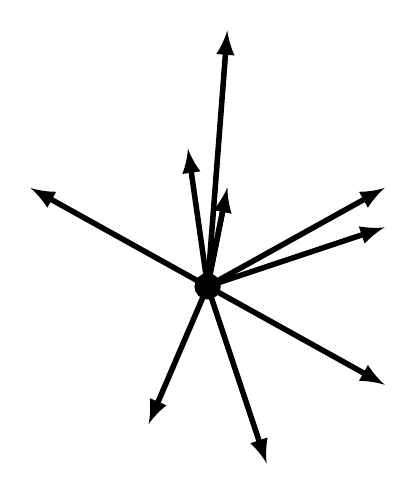
\begin{tikzpicture}[scale=0.5]
  \node (c) at (0.5, 0.5){};
  \tikzstyle{line} = [draw, -latex, line width = 2pt]
  \draw[black, fill=black] (c) circle (0.32);

  \path [line] (c) -- (0,4);
  \path [line] (c) -- (1,3);
  \path [line] (c) -- (5,2);
  \path [line] (c) -- (-4,3);
  \path [line] (c) -- (-1,-3);
  \path [line] (c) -- (1,7);
  \path [line] (c) -- (5, 3);
  \path [line] (c) -- (5,-2);
  \path [line] (c) -- (1, 3);
  \path [line] (c) -- (2,-4);

\end{tikzpicture}

  \caption{Visual representation of a histogram of oriented gradients}
  \label{ahog}
\end{figure}

The vectors can then be combined into a single graph as shown in Figure \ref{ahog}, which would be stored on a degree and magnitude basis to be fed to the classifier.

Multiple pictures with varying exposures and gain settings could also be used rather than relying on the automatic settings on the Raspberry Pi. This would have a large impact on the classification of weather types at night, as well as on the classification of bright weather types such as direct sunlight and snow.

\subsection{Closing Words}
In conclusion, time-lapse video footage was indeed able to be associated with external weather data, as was demonstrated with the creation of a reasonably accurate weather classification system. Time lapse footage created an environment in which the image was kept completely unchanged with the exception of variables which could be extracted to become features to train a classifier- something which was not obtainable with a generic image set.

With some further work and research into feature extraction and a larger dataset, this could certainly reach a high enough accuracy to be used reliable in day to day weather classification, and the work done here could be extended into other steady-position time-lapse video applications.

\addcontentsline{toc}{chapter}{Bibliography}
\bibliographystyle{ieeetr}
\bibliography{refs}{}

\chapter{Appendices}
\section{Code Extracts}

\lstset {
numbers=left,
language=java,
basicstyle=\footnotesize,
commentstyle=\color[rgb]{0,0.6,0},
keywordstyle=\color{blue},
stringstyle=\color[rgb]{0.58,0,0.82},
tabsize=2
}

\subsection{Data Harvester}
The following code was ran on the Raspberry Pi and was responsible for the data gathering and uploading.

\lstinputlisting{./snippets/DataGather.java}

\subsection{Classifier}
The following code was ran once the data was gathered to train the classifier and fill the predicted value columns on the csv file.

\lstinputlisting{./snippets/Classifier.java}

%%%%%%%%%%%%%%%%%%%%%%%%%%%%%%%%%%%%%%%%%%%
% Project Proposal
\includepdf[pages=-]{../projectplan/projectplan.pdf}

\end{document}

